
\begin{correction}  \;
Seule une \'etude des variations de la fonction assure que les bornes trouv\'ees sont bien optimales.
\begin{enumerate}
 \item $f: x\mapsto \ddp\frac{1}{1+x}  $ sur $\lbrack 0,+\infty\lbrack$.
\begin{itemize}
\item[$\bullet$] Domaine de d\'efinition: La fonction $f$ est bien d\'efinie si $1+x\not=0\Leftrightarrow x\not= -1$. Ainsi elle est en particulier bien d\'efinie sur $\lbrack 0,+\infty\lbrack$.
\item[$\bullet$] Limites aux bornes: $f(0)=1$ et $\lim\limits_{x\to +\infty} f(x)=0$ par propri\'et\'es sur les somme et quotient de limite.
\item[$\bullet$] D\'erivabilit\'e: la fonction $f$ est d\'erivable sur $\lbrack 0,+\infty\lbrack$ comme somme et quotient de fonctions d\'erivables. Et pour tout $x\geq 0$, on a: $f^{\prime}(x)=\ddp\frac{-1}{(1+x)^2}$. Ainsi: $f^{\prime}(x)<0$ pour tout $x\geq 0$. 
\item[$\bullet$] Tableau des variations:
\begin{center}
 \begin{tikzpicture}
 \tkzTabInit{ $x$          /1,%
       $f$       /2}%
     { $0$,$+\infty$}%
  \tkzTabVar{
       +/$1$            /,
         %R/          /,%
        -/$0$           /,%
                      }             
\end{tikzpicture}
\end{center}
\item[$\bullet$] \'Etude des extrema: la fonction $f$ est d\'ecroissante sur $[0,+\infty[$, et $f(0)=1$, $\lim\limits_{x\to +\infty} f(x)=0$, donc $f$ est major\'ee et minor\'ee sur $\R^+$. On obtient: $\sup_{\lbrack 0,+\infty\lbrack } f=\max_{\lbrack 0,+\infty\lbrack} f=1$ et $\inf_{\lbrack 0,+\infty\lbrack } f=0$.
\end{itemize}
%---
%\item $f: x\mapsto  \sqrt{x}-x  $ sur $\R^+$.
%\begin{itemize}
%\item[$\bullet$] Domaine de d\'efinition: La fonction $f$ est bien d\'efinie si et seulement si $x\geq 0$ at ainsi $\mathcal{D}_f=\R^+$.
%\item[$\bullet$] Limites aux bornes: $f(0)=0$ et pour tout $x>0$: $f(x)=x(-1+\ddp\frac{1}{\sqrt{x}})$: on a mis en facteur le terme dominant afin de lever l'ind\'etermination. Ainsi par propri\'et\'e sur les quotient, somme et produit de limite, on obtient: $\lim\limits_{x\to +\infty} f(x)=-\infty$.
%\item[$\bullet$] D\'erivabilit\'e: la fonction $f$ est d\'erivable si et seulement si $x>0$. Ainsi $f$ est d\'erivable sur $\R^{+\star}$ comme somme de fonctions d\'erivables. Et pour tout $x>0$: $f^{\prime}(x)=\ddp\frac{1}{2\sqrt{x}}-1=\ddp\frac{ 1-2\sqrt{x} }{2\sqrt{x}}$. Comme le d\'enominateur est strictement positif, le signe de $f^{\prime}$ ne d\'epend que du signe de $1-2\sqrt{x}$. On a: $1-2\sqrt{x}\geq 0\Leftrightarrow 1\geq 2\sqrt{x}\Leftrightarrow 1\geq 4x\Leftrightarrow x\leq \ddp\frac{1}{4}$. On a p\^{u} passer au carr\'e des deux c\^{o}t\'es tout en conservant l'\'equivalence car les deux termes sont positifs et la fonction carr\'ee est strictement croissante sur $\R^+$.
%\item[$\bullet$] Tableau des variations:
%\begin{center}
% \begin{tikzpicture}
% \tkzTabInit{ $x$          /1,%
%       $f^{\prime}(x)$   /1,
%       $f$       /2}%
%     { $0$,$\ddp\frac{1}{4}$,$+\infty$}%
%     \tkzTabLine{ ,$+$,0,$-$, }
%  \tkzTabVar{
%       -/$0$            /,
%         +/$\ddp\frac{1}{4}$          /,%
%        -/$-\infty$           /,%
%                      }                  
%\end{tikzpicture}
%\end{center}
%
%\item[$\bullet$] \'Etude des extrema: $\lim\limits_{x\to +\infty} f(x)=-\infty$ donc la fonction $f$ n'est pas minor\'ee sur $\R^+$ et elle n'admet donc ni borne inf\'erieure, ni minimum. Par contre $f$ est croissante sur $\ddp \left[0,\frac{1}{4}\right]$ et d\'ecroissante sur $\ddp \left[\frac{1}{4}, +\infty\right[$, donc la fonction $f$ est major\'ee par $\ddp\frac{1}{4}$ sur $\R^+$ et $\sup_{\lbrack 0,+\infty\lbrack } f=\max_{\lbrack 0,+\infty\lbrack} f=\ddp\frac{1}{4}$. 
%\end{itemize}
%---
\item $f: x\mapsto \cos{x}+\sin{x}$ sur $\R$.
\begin{itemize}
\item[$\bullet$] Domaine de d\'efinition: La fonction $f$ est bien d\'efinie sur $\R$ tout entier. 
\item[$\bullet$] \'Etude de la p\'eriodicit\'e: 
\begin{itemize}
\item[$\star$] $\forall x\in\mathcal{D}_f$, $x+2\pi\in\mathcal{D}_f$. 
\item[$\star$] Soit $x\in\mathcal{D}_f$: $f(x+2\pi)=\sin{(x+2\pi)}+\cos{(x+2\pi)}=\sin{x}+\cos{x}=f(x)$ en utilisant la $2\pi$ p\'eriodicit\'e des fonctions sinus et cosinus.
\end{itemize}
Ainsi la fonction $f$ est $2\pi$ p\'eriodique. Ainsi on peut restreindre l'\'etude de la fonction $f$ \`{a} tout intervalle d'amplitude $2\pi$, par exemple: $\lbrack -\pi,\pi\rbrack$.
\item[$\bullet$] D\'erivabilit\'e: la fonction $f$ est d\'erivable sur $\R$ comme somme de fonctions d\'erivables. Et pour tout $x\in\R$, $f^{\prime}(x)=-\sin{x}+\cos{x}$.\\
\noindent On \'etudie alors le signe de $f$ sur $\lbrack -\pi,\pi\lbrack$: on reconna\^{i}t une expression de la forme: $a\cos{x}+b\sin{x}$, on obtient donc: $f^{\prime}(x)=\sqrt{2}( \cos{\left(\ddp\frac{\pi}{4} \right)}\cos{x}-\sin{\left(\ddp\frac{\pi}{4} \right)}\sin{x}   )=\sqrt{2}\cos{\left( x+\ddp\frac{\pi}{4} \right)}$. \\
\noindent \'Etude du signe: on a
$$\cos{\left( x+\ddp\frac{\pi}{4} \right)} \geq 0\Leftrightarrow \exists k\in\Z,\ -\ddp\frac{\pi}{2}+2k\pi\leq x+\ddp\frac{\pi}{4}\leq \ddp\frac{\pi}{2}+2k\pi\Leftrightarrow \exists k\in\Z,\ -\ddp\frac{3\pi}{4}+2k\pi\leq x\leq \ddp\frac{\pi}{4}+2k\pi.$$
On peux alors faire un cercle trigonom\'etrique et on voit alors que sur $\lbrack -\pi,\pi\lbrack$, on a: $f^{\prime}(x)\geq 0\Leftrightarrow x\in\left\lbrack  -\ddp\frac{3\pi}{4},\ddp\frac{\pi}{4}  \right\rbrack$.  
\item[$\bullet$] Tableau des variations:
\begin{center}
 \begin{tikzpicture}
 \tkzTabInit{ $x$          /1,%
       $f^{\prime}(x)$   /1,
       $f$       /2}%
     { $-\pi$,$-\ddp\frac{3\pi}{4}$,$\ddp\frac{\pi}{4}$,$\pi$}%
     \tkzTabLine{ ,-,0,+,0,-, }
  \tkzTabVar{
       +/$-1$            /,
         -/$-\sqrt{2}$          /,%
        +/$\sqrt{2}$           /,%
        -/$-1$
                      }                   
\end{tikzpicture}
\end{center}
\item[$\bullet$] \'Etude des extrema: on a $f$ d\'ecroissante sur $\ddp \left[-\pi, -\frac{3\pi}{4}\right]$ et croissante sur $\ddp \left[-\frac{3\pi}{4}, \frac{\pi}{4}\right]$, donc $f$ admet un minimum en $\ddp-\frac{3\pi}{4}$ qui vaut $-\sqrt{2}$. De m\^eme, $f$ admet un minimum en $\ddp\frac{\pi}{4}$ qui vaut $\sqrt{2}$. La fonction $f$ est donc born\'ee sur $[-\pi, \pi]$ : elle est major\'ee par $\sqrt{2}$ et minor\'ee par 
$-\sqrt{2}$. Comme ces deux nombres sont atteints, on obtient: $\sup_{\R } f=\max_{\R} f=\sqrt{2}$ et $\inf_{\R } f=\min_{\R} f=-\sqrt{2}$. On utilise ici aussi la $2\pi$ p\'eriodicit\'e de $f$ pour passer de l'intervalle $\lbrack -\pi,\pi\lbrack$ \`{a} $\R$ tout entier.
\end{itemize}
%---
\item $f: x\mapsto \ddp\frac{1}{1+\ln{(x)}}$ sur $\lbrack 1,+\infty\lbrack$. 
\begin{itemize}
\item[$\bullet$] Domaine de d\'efinition: la fonction $f$ est bien d\'efinie si et seulement si $x>0$ et $1+\ln{x}\not= 0$. On obtient ainsi: $1+\ln{x}\not= 0\Leftrightarrow \ln{x}\not= -1\Leftrightarrow x\not= e^{-1}$ car la fonction exponentielle est strictement croissante sur $\R$. Comme $e^{-1}<1$, la fonction $f$ est donc en particulier bien d\'efinie sur $\lbrack 1,+\infty\lbrack$.
\item[$\bullet$] Limites aux bornes: on a: $f(1)=1$ et $\lim\limits_{x\to +\infty} f(x)=0$ par propri\'et\'e sur les somme et quotient de limite.
\item[$\bullet$] D\'erivabilit\'e: la fonction $f$ est d\'erivable sur son domaine de d\'efinition comme somme et quotient de fonctions d\'erivables. De plus, pour tout $x>1$, on a en particulier: $f^{\prime}(x)=\ddp\frac{-1}{x\left( 1+\ln{x} \right)^2}$. Comme on est sur $\lbrack 1,+\infty\lbrack$, on a: $x>0$. Ainsi comme un carr\'e est toujours positif, on obtient: $f^{\prime}(x)<0$.
\item[$\bullet$] Tableau des variations:
\begin{center}
 \begin{tikzpicture}
 \tkzTabInit{ $x$          /1,
       $f$       /2}%
     { $1$,$+\infty$}%
  \tkzTabVar{
       +/$1$            /,
        -/$0$
                      }                
\end{tikzpicture}
\end{center}
\item[$\bullet$] \'Etude des extrema: La fonction $f$ est ainsi major\'ee par $1$ et minor\'ee par $0$. Comme $1=f(1)$, $1$ est atteint et ainsi c'est le maximum de $f$ sur $\lbrack 1,+\infty\lbrack$: $\sup_{\lbrack 1,+\infty\lbrack } f=\max_{\lbrack 1,+\infty\lbrack} f=1$. Le nombre 0 n'est jamais atteint car c'est une limite et ainsi, on obtient $0$ est la borne inf\'erieure de $f$ sur $\lbrack 1,+\infty\lbrack$ mais il n'y a pas de minimum.
\end{itemize}
%---
\item $f: x\mapsto 5\ln{(x)}-x+\ddp\frac{6}{x}$ sur $\lbrack 1,6\rbrack$ (on donne $5\ln{(3)}\leq 6$).
\begin{itemize}
\item[$\bullet$] Domaine de d\'efinition: La fonction $f$ est bien d\'efinie si et seulement si $x>0$ et $x\not= 0$. Ainsi $\mathcal{D}_f=\R^{+\star}$ et en particulier $f$ est bien d\'efinie sur $\lbrack 1,6\rbrack$.
\item[$\bullet$] D\'erivabilit\'e: la fonction $f$ est d\'erivable sur son domaine de d\'efinition comme quotient et somme de fonctions d\'erivables. De plus, pour tout $x>0$, on a: $f^{\prime}(x)=\ddp\frac{5}{x}-1-\ddp\frac{6}{x^2}=\ddp\frac{-x^2+5x-6}{x^2}$. Le discriminant vaut $\Delta=1$ et les racines sont $2$ et $3$.  
\item[$\bullet$] Tableau des variations:
\begin{center}
 \begin{tikzpicture}
 \tkzTabInit{ $x$          /1,%
      $f^{\prime}(x)$   /1,
       $f$       /2}%
     { $0$,$2$,$3$,$+\infty$}%
    \tkzTabLine{ ,-,0,+,0,-,}
  \tkzTabVar{
       +/            /,
         -/$5\ln{2}+1$          /,%
        +/$5\ln{3}-1$           /,%
        -/
                      }
\tkzTabVal[draw]{1}{2}{0.3}{$1$}{$5$}
\tkzTabVal[draw]{3}{4}{0.45}{$6$}{$5\ln{(6)}-5$}             
\end{tikzpicture}
\end{center}
\item[$\bullet$] \'Etude des extrema: La fonction $f$ est ainsi major\'ee et minor\'ee sur $\lbrack 1,6\rbrack$. Comme $5\ln{3}-1\leq 5$, on obtient que $\sup_{\lbrack 1,6\rbrack } f=\max_{\lbrack 1,6\rbrack} f=5$. Et comme $5\ln{2}+1>5\ln{6}-5$, on a: $\inf_{\lbrack 1,6\rbrack } f=\min_{\lbrack 1,6\rbrack} f=5\ln{6}-5$.
\end{itemize}
\end{enumerate}
\end{correction}